\documentclass[a4paper, 12pt]{scrartcl}

\usepackage[utf8]{inputenc}
\usepackage[T1]{fontenc}
\usepackage[ngerman]{babel}

\usepackage{amssymb}
\usepackage{amsmath}

\usepackage{siunitx}
\usepackage{listings}
\usepackage[noline]{algorithm2e}

\usepackage{float}
\usepackage{framed}
\usepackage[hidelinks]{hyperref}

\usepackage{tikz}
\usepackage{pgfplots}
\usetikzlibrary{arrows.meta}
\pgfplotsset{compat=1.6}

\sisetup{
	separate-uncertainty,
	multi-part-units=repeat,
	locale=DE,
	scientific-notation=true,
    fixed-exponent=0,
    round-mode=places,
    round-precision=3
}

\lstset{language=C, basicstyle=\footnotesize\ttfamily, tabsize=2}

\SetAlgorithmName{Algorithmus}{}{}
\newcommand{\mycommentsty}[1]{\itshape\textcolor{gray}{#1}}
\SetCommentSty{mycommentsty}
\newcommand{\myfuncsty}[1]{\rmfamily {#1}}
\SetFuncSty{myfuncsty}
\SetStartEndCondition{ }{}{}%
\SetKw{KwTo}{in}\SetKwFor{For}{for}{\string:}{}%
\SetKwFor{While}{while}{\string:}{}%
\SetKwIF{If}{ElseIf}{Else}{if}{:}{elif}{else:}{}%
\SetKwComment{tcp}{}{}%
\SetKwComment{tcc}{}{}%
\SetKwComment{Comment}{}{}%
\AlgoDontDisplayBlockMarkers\SetAlgoNoEnd\SetNoFillComment%

\allowdisplaybreaks
\newcommand{\numberthis}{\addtocounter{equation}{1}\tag{\theequation}}
\renewcommand{\labelenumi}{(\arabic{enumi})}
\renewcommand{\labelenumii}{(\alph{enumii})}

\newcommand{\see}[1]{\hfill\emph{siehe} (\ref{#1})}

\setlength{\parindent}{0pt}

\title{Aufgabe 1\\Die Kunst der Fuge\\Dokumentation}
\author{Kamal Abdellatif}
\date{}

\begin{document}
\maketitle
\section{Obere Schranke}
Die Höhe einer Mauer von beliebigem $n$ ist nach oben beschränkt. Eine Mauer ist so breit wie die Summe der Längen $b$ aller Steine in einer Reihe. Da sich zwischen den Steinen nur die Reihenfolge ändert, entspricht die Breite jeder Reihe der Breite $w$ der Mauer.
\begin{equation}\label{eq:width}
	w = \sum_{b = 1}^n b = \frac{1}{2}n(n+1)
\end{equation}
In jeder Reihe befinden sich genau $n-1$ Fugen, da auf jeden der $n$ Steine in der Reihe genau eine Fuge folgt, mit Ausnahme des letzten Steins. Besitzt die Mauer eine Höhe $h$, so ist die Anzahl aller Fugen in der gesamten Mauer $h(n-1)$.\\
Eine Fuge nimmt entlang der Breite der Mauer eine bestimmte Position ein. Jede mögliche Position ist eine \emph{Spalte}, wobei die $i$-te Spalte den Abstand $i$ zum linken Mauerrand besitzt. Liegt auf einer Spalte eine Fuge, so ist die Spalte \emph{besetzt}.
\begin{figure}[H]
	\centering
	\begin{tikzpicture}
		\draw[ultra thick]
			(0, 0) rectangle ++(1, -1)
			(1, 0) rectangle ++(2, -1)
			(3, 0) rectangle ++(3, -1)
			(0, -1) rectangle ++(2, -1)
			(2, -1) rectangle ++(3, -1)
			(5, -1) rectangle ++(1, -1);

		\node[above] at (-.75, .25) {$i$};
		\foreach \i in {1,...,5} {
			\draw[dashed] (\i, .25) node[above] {\i} -- (\i, -2.25);
		}
	\end{tikzpicture}
	\caption{Spalten einer Mauer}
\end{figure}
Eine Mauer der Breite $w$ besitzt $w-1$ Spalten, da die erste Spalte Distanz $1$ und die letzte Spalte Distanz $w-1$ zum linken Rand aufweist.
% \newpage
Hat eine Mauer keine sich überschneidenden Fugen, so kann jede Spalte von maximal einer Fuge belegt sein. Mit jeder hinzukommenden Reihe werden $n-1$ unbelegte Spalten mit Fugen besetzt. Ist es nicht mehr möglich, eine Reihe hinzuzufügen, ohne dass eine Überschneidung entsteht, ist die höchst mögliche Mauer erreicht. Diese maximale Höhe ergibt sich somit aus dem Quotienten aus der Anzahl aller Spalten und der Anzahl von Fugen pro Reihe.
\begin{align*}
	h(n-1) &\le w-1 \numberthis\label{eq:hansatz}\\
	&\le \frac{1}{2}n(n+1) -1 \\
	h &\le \frac{\frac{1}{2}\,n(n+1)-1}{n-1} = \frac{\frac{1}{2}\,n(n-1)+n-1}{n-1} \\
	h &\le \frac{1}{2}n + 1 \numberthis\label{eq:schranke}
\end{align*}
Nur für gerade $n$ nimmt diese obere Schranke ganzzahlige Werte an. Die Schranke ist genau dann erreicht, wenn jede Spalte durch genau eine Fuge belegt ist.
\begin{equation}\label{eq:evenheight}
	h_{max} = \frac{1}{2}n + 1 \qquad (2 \mid n)
\end{equation}
Für ungerade $n$ ist die Schranke nie ganzzahlig, sodass sie nie erreicht werden kann. Demnach müssen im ungeraden Fall immer Spalten offen bleiben.
\begin{figure}[H]
	\centering
	\begin{tikzpicture}[scale=.75]
		\draw[very	thick] (0, 0) rectangle (1, 1) (1, 0) rectangle (4, 1) (4, 0) rectangle (6, 1) (6, 0) rectangle (11, 1) (11, 0) rectangle (15, 1) (0, 1) rectangle (2, 2) (2, 1) rectangle (5, 2) (5, 1) rectangle (9, 2) (9, 1) rectangle (14, 2) (14, 1) rectangle (15, 2) (0, 2) rectangle (3, 3) (3, 2) rectangle (7, 3) (7, 2) rectangle (8, 3) (8, 2) rectangle (13, 3) (13, 2) rectangle (15, 3);

		\draw[thick, dashed] (10, -.25) node[above] {} -- (10, 3.25);
		\draw[thick, dashed] (12, -.25) node[above] {} -- (12, 3.25);
	\end{tikzpicture}
	\caption{Offene Spalten bei ungeraden $n$}
\end{figure}
Die größte erreichbare Höhe $h_{max}$ für ungerade $n$ ist gleich der größten ganzen Zahl unter der Schranke. Aus Gleichung (\ref{eq:schranke}) ergibt sich
\begin{equation}\label{eq:oddheight}
	h_{max} = \frac{1}{2}(n-1)+1 = \frac{1}{2}(n+1) \qquad (2 \nmid n)
\end{equation}
Wird diese Höhe erreicht, so ist die Anzahl $r$ der noch offenen Spalten die Differenz aus der Anzahl aller Spalten $w-1$ und der Anzahl besetzter Spalten $h_{max}(n-1)$.
\begin{align*}
	r &= (w-1) - h_{max}(n-1) \\
	&= \left( \frac{n(n+1)}{2} - 1 \right) - \frac{n+1}{2}\,(n-1) \\
	&= \frac{(n+1)(n-1)+n-1}{2}-\frac{(n+1)(n-1)}{2} \\
	r &= \frac{1}{2}(n-1) \qquad (2 \nmid n) \numberthis\label{eq:offen}
\end{align*}
Für eine Mauer ungeraden $n$ ohne Überschneidungen müssen mindestens $r = \frac{1}{2}(n-1)$ Spalten offen bleiben.
\section{Algorithmus}
\label{sec:algorithmus}
\subsection{Vorbetrachtung}
\label{subsec:vorbetrachtung}
Das Problem wird mit Backtracking gelöst. Es wird davon ausgegangen, dass die nach der oberen Schranke (\ref{eq:schranke}) gegebene größtmögliche Höhe $h = h_{max}$ immer erreichbar ist. Um eine Mauer $n$ zu lösen, wird von einer leeren Mauer der Dimensionen $w \times h$ ausgegangen. Ziel des Backtracking ist es, diese Mauer Stein für Stein zu füllen, ohne dass sich Fugen überschneiden.

Eine Mauer $W = \left\{ R_1,\ \dots,\ R_h \right\}$ besteht aus $h$ Reihen $R$. Während der Konstruktion der Mauer sind die Reihen nur teilweise gefüllt. Eine Reihe $R = \left\{ b_1,\ \dots,\ b_k \right\}$ enthält $k \leq n$ Steine einer bestimmten Länge $b$. Ein Stein $b_i$ ist der $i$-te Stein von links innerhalb der Reihe. Nur die Steine $\Sigma = \left\{ 1,\ \dots,\ n \right\}$ können in einer Reihe $R \subseteq \Sigma$ enthalten sein.

Jede Reihe $R$ besitzt eine Länge $\ell(R)$. Diese Länge ergibt sich aus der Summe aller in $R$ enthaltenen Steinlängen.
\begin{equation}\label{eq:laenge}
	\ell(R) = \sum_{b_i \in R} b_i
\end{equation}
Die Reihe endet in der $\ell$-ten Spalte. Diese Spalte wird als \emph{Endpunkt} der Reihe bezeichnet.
\begin{figure}[H]
	\centering
	\begin{tikzpicture}[scale=1.1]
		\draw[gray, dashed]
			(0, -1) rectangle ++(2, -1)
			(2, -1) rectangle ++(3, -1)
			(4, -2) rectangle ++(2, -1)
			(0,  0) rectangle ++(10, -3);
		\draw[very thick]
			(0, 0) rectangle ++(1, -1)
			(1, 0) rectangle ++(2, -1)
			(3, 0) rectangle ++(4, -1);

		\node at (-.5, -.5) {$R_1$};
		\node[gray] at (-.5, -1.5) {$R_2$};
		\node[gray] at (-.5, -2.5) {$R_3$};

		\node at (.5, -.5)  {{\small$b_1=1$}};
		\node at (2, -.5)   {{\small$b_2=2$}};
		\node at (5, -.5) {{\small$b_3=4$}};
		\draw[|-|, very thick] (0, -1.3) to (7, -1.3) node[right] {$\ell = 7$};
		\node at (8, -.5) {$k = 3$};
	\end{tikzpicture}
	\caption{Bezeichnungen}
\end{figure}
\subsection{Gerade Fälle}
In der Lösung einer Mauer mit geraden $n$ ist jede Spalte durch genau eine Fuge besetzt. Um diese Lösung zu konstruieren, werden die Spalten nacheinander von links nach rechts mit Fugen aufgefüllt. Mit jedem Backtracking-Schritt wird eine Spalte gefüllt. Dazu wird ein Stein direkt an das rechte Ende einer Reihe angelegt.
\begin{figure}[H]
	\centering
	\begin{tikzpicture}[scale=.75]
		\draw[very thick] (0, 0) rectangle (15, 3);
		\draw[very thick, fill=white] (0, 0) rectangle (1, 1) (1, 0) rectangle (4, 1) (4, 0) rectangle (6, 1) (0, 1) rectangle (2, 2) (2, 1) rectangle (5, 2) (0, 2) rectangle (3, 3);
		\draw[very thick, gray, fill=white] (3.1, 2.1) rectangle (7.1, 3.1);

		\node at (-.5, 2.5) {$R$};

		\draw[|-{Latex}, thick] (0, -.5) to ++(7, 0) node[right] {$s$};
		\draw[thick, dashed] (7, -.5) -- (7, 3.5);
		\draw[|-|, thick] (0, 3.5) to node[above] {$\ell(R)$} ++(3, 0);
		\draw[|-|, thick] (3, 4) to node[above] {$b'$} ++(4, 0);
	\end{tikzpicture}
	\caption{Anlegen eines Steins}
\end{figure}
Soll eine Reihe $R$ zu der Spalte $s$ erweitert werden, muss ein Stein bestimmter Länge $b'$ hinzugefügt werden. Da die Reihe nach Anfügen des Steins in Spalte $s$ endet, ist der neue Stein genau so lang sein wie die Differenz zwischen $s$ und dem aktuellem Ende der Reihe $\ell$. Dabei darf $b'$ noch nicht in $R$ enthalten sein, da es sonst zu einer Wiederholung kommen würde.
\begin{equation}\label{eq:bprime}
	b' = s-\ell(R) \qquad (b' \in \Sigma \backslash R)
\end{equation}
Nach Anfügen des Steins hat sich in der $R$ die Anzahl $k$ von Steinen um eins erhöht und die Länge um $b'$ vergrößert. Da die Spalte $s$ nun durch eine Fuge gefüllt ist, wird als nächstes die darauf folgende Spalte $s+1$ gefüllt. Dieser Vorgang wird als \emph{Schritt} bezeichnet.
\begin{align}\label{eq:trans}
	R' &= R\,\cup\,\{b'\} & \ell' &= \ell + b' & s' &= s+1
\end{align}
Durch diese Vorgehensweise wird jede Spalte durch genau eine Fuge besetzt und in keiner Reihe wird ein Stein wiederholt. Wurden alle Reihen vollständig gefüllt, so ist eine Lösung gefunden worden.

Das Backtracking öffnet einen neuen Suchzweig für jede mögliche Reihe, die zum Füllen der nächsten Spalte gewählt werden kann. Eine Reihe $R$ kann genau dann gewählt werden, wenn der benötigte Stein $b'$ noch nicht in $R$ enthalten ist. Ist der Stein doch enthalten, oder sein Länge überschreitet $n$, so handelt es sich um eine \emph{Kollision}. Ist keine Reihe mehr möglich, so muss der gesamte Suchzweig verworfen werden.

Das Backtracking geht in Tiefensuche vor und wird rekursiv implementiert. Jeder Rekursionsschritt besteht aus drei Schritten:
\begin{enumerate}
	\item Der zu untersuchende Schritt wird ausgeführt: Der Stein wird an die entsprechende Reihe angefügt und die aktuelle Spalte inkrementiert.
	\item Alle Folgeschritte werden untersucht. Dazu wird durch alle möglichen Reihen iteriert. Der Erfolg des aktuellen Schrittes hängt davon ab, ob mindestens eine davon erfolgreich war.
	\item Die unternommenen Änderungen werden rückgängig gemacht.
\end{enumerate}
Sobald eine Lösung gefunden wurde, wird die Suche abgebrochen. War eine der Möglichkeiten erfolgreich, so werden weitere Möglichkeiten außer acht gelassen, und der Erfolg wird sofort zurückgegeben.

Für den vollständigen Algorithmus in Pseudocode siehe Anhang (\ref{alg:even}).

\subsection{Ungerade Fälle}
Für ungerade $n$ ist nicht mehr gegeben, dass jede Spalte durch genau eine Fuge besetzt wird. Genauer, nach Gleichung (\ref{eq:offen}) bleiben in einer maximalen Lösung genau $r = \frac{1}{2}(n-1)$ Spalten offen.

Um das Backtracking auf alle Fälle zu erweitern, wird die Möglichkeit hinzugefügt, bestimmte Spalten auszulassen. Ist es in einem ungeraden Fall während des Backtracking nicht möglich, die direkt folgende Spalte $s$ zu füllen, so kann diese Spalte \emph{übersprungen} werden. Dazu wird nicht versucht, die Spalte $s$ zu füllen, sondern die darauf folgende Spalte $s+1$.
\begin{figure}[H]
	\centering
	\begin{tikzpicture}[scale=.75]
		\draw[very thick] (0, 0) rectangle ++(4, 1)
		                  (4, 0) rectangle ++(2, 1)
		                  (0, 1) rectangle ++(2, 1)
		                  (2, 1) rectangle ++(3, 1)
		                  (0, 2) rectangle ++(1, 1)
		                  (1, 2) rectangle ++(2, 1)
		                  (3, 2) rectangle ++(4, 1)
		                  (0, 0) rectangle (15, 3);
		\draw[very thick, gray] (6.1, .1) rectangle ++(3, 1);
		\draw[thick, dashed] (8, 3.25) to ++ (0, -3.5) node[below] {$s\vphantom{s+1}$};
		\draw[thick, dashed] (9, -.25) to ++ (0,  3.5) node[above] {$s+1$};
	\end{tikzpicture}
	\caption{Überspringen einer Spalte}
\end{figure}
Ist es auch nicht möglich, die Spalte $s+1$ zu füllen, so wird diese ebenfalls übersprungen. Es ist demnach möglich, auch mehrere Spalten in einem Schritt zu überspringen. Sei $z$ die Anzahl von übersprungenen Spalten in einem Schritt.

Während des Backtrackings soll $r$ die Anzahl von Spalten darstellen, die noch übersprungen werden können. Anfänglich ist $r$ die durch Gleichung (\ref{eq:offen}) gegebene Insgesamtanzahl, insofern $n$ ungerade ist. Handelt es sich um einen geraden Fall, so dürfen keine Spalten übersprungen werden, womit $r=0$.
\begin{equation}\label{eq:sprung}
	r =
	\begin{cases}
		0 &\qquad (2 \mid n)\\
		\frac{1}{2}(n-1) &\qquad (2 \nmid n)
	\end{cases}
\end{equation}
Wurden $z$ Spalten übersprungen, so verringert sich $r$ um diese Zahl. Es können mindestens $0$ und maximal $r$ Spalten in einem Schritt übersprungen werden. Da nun nicht immer die direkt folgende Spalte als betrachtet wird, müssen die Gleichungen (\ref{eq:bprime}) und (\ref{eq:trans}) für den Übergang zum nächsten Schritt erweitert werden.
\begin{gather}
	b' = s + z -\ell(R) \qquad (b' \in \Sigma \backslash R \ \wedge\ 0 \le z \le r) \label{eq:bprimeodd}\\
	R' = R\,\cup\,\{b'\} \qquad \ell' = \ell + b' \qquad s' = s+z+1 \qquad r' = r - z \label{eq:transodd}
\end{gather}
Ein Schritt setzt sich nun zusammen aus einer Reihe $R \in W$ und einer Anzahl von Sprüngen $z \in Z$ mit $Z = \left\{ 0,\ \dots,\ r \right\}$. Die Menge aller Folgeschritte ist die Menge von allen Kombinationen $W \times Z$. Dazu werden die Iterationen über die Reihen und über die Sprunglängen geschachtelt. Die äußere Iteration geht über $z$ aufsteigend. Es werden demnach immer zuerst die Möglichkeiten mit der geringsten Anzahl von Sprüngen betrachtet. Für den erweiterten Algorithmus siehe Anhang (\ref{alg:all}).
\subsection{Suchheuristik}
\label{subsec:heuristik}
Mit dem Backtracking wird ein Suchbaum abgelaufen. Jeder Knoten in diesem Baum stellt einen Füllzustand der Wand dar, während ein Schritt von einem Zustand zum nächsten eine Kante ist. Ist kein Schritt von einem Knoten aus mehr möglich, so handelt es sich um eine \emph{Sackgasse}. Ist die Mauer vollständig gefüllt, so ist der zugehörige Zustands-Knoten eine \emph{Lösung}. Alle Blätter des Baums sind entweder Sackgassen oder Lösungen.
\begin{figure}[H]
	\centering
	\begin{tikzpicture}[scale=.75, y=8mm]
		\def\checkmark{\tikz\fill[scale=0.4](0, .35) -- (.25, 0) -- (.6, .7) -- (.25, .15) -- cycle;} 
		\tikzstyle{node}=[draw, thick, circle, inner sep=0pt, minimum width=5mm]
		\large
		\node[node] (a) at (0, 6) {};
		\node[node] (b1) at (-4, 4) {};
		\node[node] (b2) at (0, 4) {};
		\node[node] (b3) at (4, 4) {};
		\node[node] (c11) at (-5, 2) {};
		\node[node] (c12) at (-4, 2) {};
		\node[node] (c13) at (-3, 2) {$\times$};
		\node[node] (c22) at (0, 2) {};
		\node[node] (c23) at (1, 2) {$\times$};
		\node[node] (c33) at (4, 2) {$\times$};
		\node[node] (d111) at (-7, 0) {$\times$};
		\node[node] (d112) at (-6, 0) {$\times$};
		\node[node] (d113) at (-5, 0) {$\times$};
		\node[node] (d122) at (-4, 0) {$\times$};
		\node[node] (d221) at (-1, 0) {$\times$};
		\node[node] (d222) at (0, 0) {\checkmark};
		\draw[-{latex}, thick] (a) edge (b1) (a) edge (b2) (a) edge (b3)
		                 (b1) edge (c11) (b1) edge (c12) (b1) edge (c13)
		                 (b2) edge (c22) (b2) edge (c23)
		                 (b3) edge (c33)
		                 (c11) edge (d111) (c11) edge (d112) (c11) edge (d113)
		                 (c12) edge (d122)
		                 (c22) edge (d221) (c22) edge (d222);
	\end{tikzpicture}
	\caption{Suchbaum}
\end{figure}
Das Backtracking geht den gesamten Baum ab, bis eine Lösung gefunden wurde. Die Größe des Baums, der bis zur ersten gefundenen Lösung betrachtet werden musste, ist maßgebend für die Laufzeit der Suche. Dabei ist die Reihenfolge entscheidend, in der die einzelnen Möglichkeiten abgelaufen werden.
\par
\begin{minipage}{.45\textwidth}
	\begin{figure}[H]
		\begin{tikzpicture}[scale=.75, x=9mm, y=8mm]
			\def\checkmark{\tikz\fill[x=4mm, y=4mm](0, .35) -- (.25, 0) -- (.6, .7) -- (.25, .15) -- cycle;} 
			\tikzstyle{node}=[draw, thick, circle, inner sep=0pt, minimum width=5mm]
			\large
			\node[node] (a) at (0, 6) {};
			\node[node] (b1) at (-4, 4) {};
			\node[node] (b2) at (0, 4) {};
			\node[node, opacity=.2] (b3) at (4, 4) {};
			\node[node] (c11) at (-5, 2) {};
			\node[node] (c12) at (-4, 2) {};
			\node[node] (c13) at (-3, 2) {$\times$};
			\node[node] (c22) at (0, 2) {};
			\node[node, opacity=.2] (c23) at (1, 2) {$\times$};
			\node[node, opacity=.2] (c33) at (4, 2) {$\times$};
			\node[node] (d111) at (-7, 0) {$\times$};
			\node[node] (d112) at (-6, 0) {$\times$};
			\node[node] (d113) at (-5, 0) {$\times$};
			\node[node] (d122) at (-4, 0) {$\times$};
			\node[node] (d221) at (-1, 0) {$\times$};
			\node[node] (d222) at (0, 0) {\checkmark};
			\draw[-{latex}, thick] (a) edge (b1) (a) edge (b2) (a) edge[opacity=.2] (b3)
			                 (b1) edge (c11) (b1) edge (c12) (b1) edge (c13)
			                 (b2) edge (c22) (b2) edge[opacity=.2] (c23)
			                 (b3) edge[opacity=.2] (c33)
			                 (c11) edge (d111) (c11) edge (d112) (c11) edge (d113)
			                 (c12) edge (d122)
			                 (c22) edge (d221) (c22) edge (d222);
		\end{tikzpicture}
		\caption{Betrachteter Teilbaum von links nach rechts}
	\end{figure}
\end{minipage}
\hfill
\begin{minipage}{.45\textwidth}
	\begin{figure}[H]
		\begin{tikzpicture}[scale=.75, x=9mm, y=8mm]
			\def\checkmark{\tikz\fill[x=4mm, y=4mm](0, .35) -- (.25, 0) -- (.6, .7) -- (.25, .15) -- cycle;} 
			\tikzstyle{node}=[draw, thick, circle, inner sep=0pt, minimum width=5mm]
			\tikzstyle{node_}=[draw, thick, circle, inner sep=0pt, minimum width=5mm, opacity=.2]
			\large
			\node[node] (a) at (0, 6) {};
			\node[node_] (b1) at (-4, 4) {};
			\node[node] (b2) at (0, 4) {};
			\node[node] (b3) at (4, 4) {};
			\node[node_] (c11) at (-5, 2) {};
			\node[node_] (c12) at (-4, 2) {};
			\node[node_] (c13) at (-3, 2) {$\times$};
			\node[node] (c22) at (0, 2) {};
			\node[node] (c23) at (1, 2) {$\times$};
			\node[node] (c33) at (4, 2) {$\times$};
			\node[node_] (d111) at (-7, 0) {$\times$};
			\node[node_] (d112) at (-6, 0) {$\times$};
			\node[node_] (d113) at (-5, 0) {$\times$};
			\node[node_] (d122) at (-4, 0) {$\times$};
			\node[node_] (d221) at (-1, 0) {$\times$};
			\node[node] (d222) at (0, 0) {\checkmark};
			\draw[-{latex}, thick, opacity=.2] (a) edge (b1)  
			                 (b1) edge (c11) (b1) edge (c12) (b1) edge (c13)
			                 (c11) edge (d111) (c11) edge (d112) (c11) edge (d113)
			                 (c12) edge (d122)
			                 (c22) edge (d221);
			\draw[-{latex}, thick]
			                 (a) edge (b2)
			                 (a) edge (b3)
			                 (b2) edge (c22)
			                 (b2) edge (c23)
			                 (b3) edge (c33)
			                 (c22) edge (d222);
		\end{tikzpicture}
		\caption{Betrachteter Teilbaum von rechts nach links}
	\end{figure}
\end{minipage}
\\\\\\
Um die Laufzeit der Suche zu verringern, wird eine Suchheuristik angewendet, welche die Reihenfolge der betrachteten Möglichkeiten beeinflusst. Eine solche Heuristik sollte die Schritte zuerst wählen, die eine höhere Wahrscheinlichkeit haben, zielführend zu sein. So verringert sich die durchschnittliche Größe des betrachteten Teilbaums. Ausschlaggebend für diese Größe ist unter Anderem die Anzahl von vorgekommenen Kollisionen.
\\\\
Werden die Reihen immer in der gleichen Reihenfolge betrachtet, entsteht eine Ungleichgewichtung in den Steinlängen. Es wird immer versucht, die nächste Fuge zuerst in den oben liegenden Reihen zu setzen. So werden tendenziell mehr Fugen in den oberen Reihen und weniger in den unteren gesetzt. Eine höhere Dichte an Fugen führt zu kleineren Steinlängen. Daher füllen sich die oberen Reihen zuerst mit kurzen Steinlängen und die unteren mit Langen. Dieses Verhalten erzeugt eine erhöhte Anzahl von Kollisionen: Werden beispielsweise in den oberen Reihen kurze Steinlängen bevorzugt, so ist es beim Anfügen eines weiteren kurzen Steins wahrscheinlicher, dass dieser schon verwendet wurde. Gleiches gilt für die unteren Reihen mit langen Steinen.

Werden die Fugen anfänglich nur oben gesetzt, so können untere Reihen sogar so weit zurückfallen, dass selbst der längste Stein nicht zum Auffüllen ausreicht. Da die unteren Reihen erst dann betrachtet werden, wenn alle Oberen keine Kapazität mehr haben, werden diese Suchzweige erst sehr spät abgebrochen. Dies führt zu vollständigen Suchzweigen, die verworfen werden müssen, da die unteren Reihen von Anfang an nicht mehr füllbar waren.
\begin{figure}[H]
	\centering
	\begin{tikzpicture}[scale=.75]
		\draw[ultra thick] (0, 1) rectangle ++(4, 1)
		                  (4, 1) rectangle ++(3, 1)
		                  (7, 1) rectangle ++(1, 1)
		                  (0, 2) rectangle ++(2, 1)
		                  (2, 2) rectangle ++(3, 1)
		                  (5, 2) rectangle ++(4, 1)
		                  (0, 3) rectangle ++(1, 1)
		                  (1, 3) rectangle ++(2, 1)
		                  (3, 3) rectangle ++(3, 1)
		                  (6, 3) rectangle ++(4, 1)
		                  (0, 0) -- (0, 4) -- (15, 4)
		                  (0, 0) -- (15, 0);
		\draw[dashed, very thick] (11, -.25) -- (11, 4.25);
	\end{tikzpicture}
	\caption{erste Sackgasse im Backtracking für $n=6$}\label{fig:sackgasse}
\end{figure}
Im Beispiel von Abbildung (\ref{fig:sackgasse}) können die oberen drei Reihen nicht besetzt werden, da die benötigten Steine schon verbaut sind. Allerdings sind schon die ersten zehn Spalten besetzt, sodass seit vier Schritten schon die unterste Reihe nicht mehr besetzbar war.
\\\\
Im Anhang Abbildung (\ref{fig:kollisionen}) und Tabelle (\ref{fig:statistik}) wird die Kollisionshäufigkeit genauer statistisch untersucht. Die Beobachtungen unterstützen die obigen Vorhersagen.
\newpage
Die gewählte Heuristik wirkt diesen Effekten entgegen.
\begin{framed}
	\centering
	\textsc{\raggedleft Suchheuristik}\\
	Reihen werden nach aufsteigender Länge betrachtet.
\end{framed}
Durch Ordnung nach aufsteigender Länge werden immer zuerst die kürzesten Reihen betrachtet. So bleibt die Längenverteilung innerhalb der Reihen gleichmäßig, da keine Reihe zurückfallen kann.
\begin{figure}[H]
	\centering\sffamily
\begin{tikzpicture}[scale=.5]
	\path (-1, -1) to (13, -1) to (13, 5) to (-1, 5) to cycle;  % phantom
	\node at (6, -1) {(a)};
	\draw[very thick]
		(0, 0) rectangle ++(5, 1)
		(5, 0) rectangle ++(4, 1)
		(0, 1) rectangle ++(2, 1)
		(2, 1) rectangle ++(6, 1)
		(0, 2) rectangle ++(1, 1)
		(1, 2) rectangle ++(2, 1)
		(3, 2) rectangle ++(4, 1)
		(0, 3) rectangle ++(4, 1)
		(4, 3) rectangle ++(2, 1)
		(0, 0) -- (0, 4) -- (12, 4)
		(0, 0) -- (12, 0);
\end{tikzpicture}
\begin{tikzpicture}[scale=.5]
	\path (-1, -1) to (13, -1) to (13, 5) to (-1, 5) to cycle;  % phantom
	\node at (6, -1) {(b)};
	\draw[very thick]
		(0, 0) rectangle ++(5, 1)
		(5, 0) rectangle ++(4, 1)
		(0, 1) rectangle ++(2, 1)
		(2, 1) rectangle ++(6, 1)
		(0, 2) rectangle ++(1, 1)
		(1, 2) rectangle ++(2, 1)
		(3, 2) rectangle ++(4, 1)
		(0, 3) rectangle ++(4, 1)
		(4, 3) rectangle ++(2, 1)
		(0, 0) -- (0, 4) -- (12, 4)
		(0, 0) -- (12, 0);
	\draw[very thick, gray] (7.2, 2.2) rectangle ++(3, 1);
\end{tikzpicture}
\begin{tikzpicture}[scale=.5]
	\path (-1, -1) to (13, -1) to (13, 5) to (-1, 5) to cycle;  % phantom
	\node at (6, -1) {(c)};
	\draw[very thick, opacity=.2, dashed]
		(0, 0) rectangle ++(5, 1)
		(5, 0) rectangle ++(4, 1)
		(0, 1) rectangle ++(2, 1)
		(2, 1) rectangle ++(6, 1)
		(0, 2) rectangle ++(1, 1)
		(1, 2) rectangle ++(2, 1)
		(3, 2) rectangle ++(4, 1)
		(0, 3) rectangle ++(4, 1)
		(4, 3) rectangle ++(2, 1);
	\draw[very thick]
		(0, 2) rectangle ++(1, 1)
		(1, 2) rectangle ++(2, 1)
		(3, 2) rectangle ++(4, 1)
		(7, 2) rectangle ++(3, 1);
	\path[-{latex}, very thick] (-.2, 2.5) edge[bend right=40] (-.2, -.5);
\end{tikzpicture}
\begin{tikzpicture}[scale=.5]
	\path (-1, -1) to (13, -1) to (13, 5) to (-1, 5) to cycle;  % phantom
	\node at (6, -1) {(d)};
	\draw[very thick]
		(0, 0) rectangle ++(1, 1)
		(1, 0) rectangle ++(2, 1)
		(3, 0) rectangle ++(4, 1)
		(7, 0) rectangle ++(3, 1)
		(0, 1) rectangle ++(5, 1)
		(5, 1) rectangle ++(4, 1)
		(0, 2) rectangle ++(2, 1)
		(2, 2) rectangle ++(6, 1)
		(0, 3) rectangle ++(4, 1)
		(4, 3) rectangle ++(2, 1)
		(0, 0) -- (0, 4) -- (12, 4)
		(0, 0) -- (12, 0);
\end{tikzpicture}
	\caption{Umordnung nach Anfügen eines Steins}
\end{figure}
Das Anfügen eines Steins verlängert die gewählte Reihe. Da bis zu einer bisher ungefüllten Spalte aufgefüllt wird, ist die Reihe nach Auffüllen die längste Reihe der Mauer. Demnach rutscht die gewählte Reihe immer an das Ende der Ordnung. Die Reihenfolge der restlichen Reihen bleibt erhalten. War ein Schritt nicht erfolgreich, müssen die unternommenen Veränderungen für das Backtracking rückgängig gemacht werden. Die gewählte Reihe muss demnach wieder an die vorherige Position in der Ordnung gesetzt werden.
\newpage
\section{Implementation}
\subsection{Datenstrukturen}
\label{subsec:datenstrukturen}
Der in Sektion (\ref{sec:algorithmus}) beschriebene Algorithmus greift auf abstrakte Datenstrukturen wie Mengen zurück. Eine Mauer wird in jedem Zustand während der Suche durch folgende Eigenschaften charakterisiert:
\begin{enumerate}
	\itemsep-2pt
	\item die gegebene Zahl $n$
	\item eine Breite $w$ \see{eq:width}
	\item eine maximale Höhe $h$ \hfill \emph{siehe} (\ref{eq:evenheight}, \ref{eq:oddheight})
	\item die Anzahl von noch möglichen Sprüngen $r$ \see{eq:sprung}
	\item die zu füllende Spalte $s$
	\item eine Menge $W$ von Reihen $R$ mit
	\begin{enumerate}
		\item allen beinhalteten Steinen $b$ als Element
		\item einer bestimmten Länge $\ell(R)$ \see{eq:laenge}
	\end{enumerate}
	\item einer Reihenfolge für Reihen in $W$  \hfill \emph{siehe} Sektion \ref{subsec:heuristik}
\end{enumerate}
Die Eigenschaften (1) bis (5) sind als natürliche Zahlen darstellbar. Die Reihe $R$ muss innerhalb der Suche drei Operationen mit einem Stein $b$ unterstützen: Einfügen, Entfernen und Test nach Beinhaltung.
\begin{align*}
 	R &\leftarrow R\cup\{b\} & R &\leftarrow R\backslash\{b\} & (b &\in R)
\end{align*}
Als Datenstruktur wird für jede Reihe ein boolesches Array $usedBricks[n]$ verwendet. Das $i$-te Element $usedBricks[i]$ sagt dabei aus, ob der Stein der Länge $b=i+1$ enthalten ist. Das Hinzufügen beziehungsweise Entfernen wird durch die Änderung des Wertes des jeweiligen Elements erzielt. Alle Operationen benötigen dabei eine Laufzeitkomplexität von $\mathcal{O}(1)$.
\begin{figure}[H]
	\centering
	\begin{tabular}{rcc}
		Operation & \hspace{1cm} Menge $R$ \hspace{1cm} & Array $usedBricks$ \\
		\hline\\
		Einfügen & $R \leftarrow R\cup\{b\}$ & $usedBricks[b-1] \leftarrow 1$ \\\\
		Entfernen & $R \leftarrow R\backslash\{b\}$ & $usedBricks[b-1] \leftarrow 0$ \\\\
		Beinhaltung & $(b \in R)$ & $(usedBricks[b-1])$
	\end{tabular}
\end{figure}
Alle booleschen Arrays werden in einem Array $wall[h]$ zusammengefasst. Der entsprechende Index innerhalb von $wall[\,]$ identifiziert jede Reihe eindeutig und ist unveränderlich.

Durch die eindeutige Zuordnung jeder Reihe mit einem Index kann die in Sektion (\ref{subsec:heuristik}) beschriebene Reihenfolge durch eine Liste $order[h]$ ausgedrückt werden. Der Wert jedes Elements $order[i]$ entspricht dem Index der $i-ten$ Reihe innerhalb der Reihenfolge. Die kürzeste Reihe liegt in $order[0]$.

Da die Ordnung veränderlich ist, ist eine dynamische Datenstruktur angebracht. Diese muss effizient folgende Operationen implementieren:
\begin{enumerate}
	\itemsep-2pt
	\item Einfügen eines Elements $d$
	\item Entfernen eines Elements $d$
	\item Anfügen eines Elements $d$ am Ende
	\item Entfernen des letzten Elements
	\item Iteration durch alle Elemente
\end{enumerate}
Es werden Double-Linked-Lists verwendet, welche alle genannten Operationen (bis auf Iteration) in $\mathcal{O}(1)$ ermöglichen. Das Einfügen an einem bestimmten Index benötigt eigentlich $\mathcal{O}(n)$, da die Liste erst durchgegangen werden muss.

Die Reihenfolge wird am Anfang und Ende von jedem Schritt verändert. Dabei wird die aktuelle Reihe innerhalb der Iteration an das Ende gesetzt, und wieder an die ursprüngliche Position zurück. Dabei ist immer der Zeiger der Reihe innerhalb der Iteration (\textsf{R}) und der Zeiger auf das Ende der Reihenfolge (\textsf{E}) bekannt. Es können demnach statt den Indices auch die Zeiger auf die Elemente verwendet werden, was eine lineare Suche erübrigt.
\begin{figure}[H]
	\centering\large\sffamily%
\tikzstyle{box}=[draw, thick, rectangle, inner sep=0pt, minimum width=1cm, minimum height=1cm, anchor=south west]
\begin{tikzpicture}
	\draw (-1.2, -1.2) rectangle (6.2, 2.2);
	\node at (-.6, 1.6) {\small(a)};
	\node[box] at (0, 0) {2};
	\node[box] at (1, 0) {1};
	\node[box] at (2, .1) {4};
	\node[box] at (3, 0) {5};
	\node[box] at (4, 0) {3};
	\node[box, opacity=.2] at (5, 0) {4};
	\draw[thick] (2.5, 0) -- ++(-60:.5) -- ++(180:.5) -- cycle node[below=4mm] {R};
	\draw[thick] (4.5, 0) -- ++(-60:.5) -- ++(180:.5) -- cycle node[below=4mm] {E};
	\draw[thick, opacity=.2] (5.5, 0) -- ++(-60:.5) -- ++(180:.5) -- cycle node[below=4mm] {E};
	\path[-{latex}, ultra thick] (2.5, 1.2) edge[bend left=50] (5.5, 1.1);
\end{tikzpicture}
\begin{tikzpicture}
	\draw (-1.2, -1.2) rectangle (6.2, 2.2);
	\node at (-.6, 1.6) {\small(b)};
	\node[box] at (0, 0) {2};
	\node[box] at (1, 0) {1};
	\node[box] at (2, 0) {5};
	\node[box] at (3, 0) {3};
	\node[box] at (4, 0) {4};
	\draw[thick] (2.5, 0) -- ++(-60:.5) -- ++(180:.5) -- cycle node[below=4mm] {R};
	\draw[thick] (4.5, 0) -- ++(-60:.5) -- ++(180:.5) -- cycle node[below=4mm] {E};
\end{tikzpicture}\par\vspace{1mm}%
\begin{tikzpicture}
	\draw (-1.2, -1.2) rectangle (6.2, 2.2);
	\node at (-.6, 1.6) {\small(c)};
	\node[box] at (0, 0) {2};
	\node[box] at (1, 0) {1};
	\node[box] at (2.2, 0) {5};
	\node[box] at (3.2, 0) {3};
	\node[box] at (4.2, 0.1) {4};
	\draw[thick] (2.7, 0) -- ++(-60:.5) -- ++(180:.5) -- cycle node[below=4mm] {R};
	\draw[thick] (4.7, .1) -- ++(-60:.5) -- ++(180:.5) -- cycle node[below=4mm] {E};
	\path[-{latex}, ultra thick] (4.7, 1.2) edge[bend right=50] (2.1, 1.1);
\end{tikzpicture}
\begin{tikzpicture}
	\draw (-1.2, -1.2) rectangle (6.2, 2.2);
	\node at (-.6, 1.6) {\small(d)};
	\node[box] at (0, 0) {2};
	\node[box] at (1, 0) {1};
	\node[box] at (2, 0) {4};
	\node[box] at (3, 0) {5};
	\node[box] at (4, 0) {3};
	\draw[thick] (2.5, 0) -- ++(-60:.5) -- ++(180:.5) -- cycle node[below=4mm] {R};
	\draw[thick] (4.5, 0) -- ++(-60:.5) -- ++(180:.5) -- cycle node[below=4mm] {E};
\end{tikzpicture}
	\caption{Zeiger in der Linked-List während eines Schrittes}
\end{figure}\vspace{-6pt}
Die Längen $\ell(R)$ müssen nicht erst als Summe (\emph{siehe} \ref{eq:laenge}) der Steinlängen errechnet werden, da dies $\mathcal{O}(n)$ benötigen würde. Stattdessen werden die Längen in einem Array $endpoints[h]$ gespeichert, wobei $endpoints[i]$ die Länge $\ell(R)$ der Reihe mit Index $i$ darstellt. Am Anfang sind alle Reihen leer, sodass $endpoints$ mit 0 initialisiert wird. Wird ein Stein der Länge $b$ in der Reihe $R$ hinzugefügt oder entfernt, wird dies auf die Länge addiert beziehungsweise subtrahiert. Dies geschieht in $\mathcal{O}(1)$.
\enlargethispage{3em}
\begin{figure}[H]
	\centering
	\begin{tabular}{rcc}
		Operation & \hspace{1cm} Menge $R$ \hspace{1cm} & Array $endpoints$ \\
		\hline
		Einfügen & $R \leftarrow R\cup\{b\}$ & $endpoints[i] \leftarrow endpoints[i] + b$ \\
		Entfernen & $R \leftarrow R\backslash\{b\}$ & $endpoints[i] \leftarrow endpoints[i] - b$
	\end{tabular}
\end{figure}
\section{Laufzeit}
Die Laufzeit des Programms hängt von der Größe des betrachteten Suchbaums ab. Liegen die Lösungen ungünstig, kann im Worst-Case-Szenario die erste Lösung erst am Ende des Suchbaums gefunden werden. Das asymptotische Verhalten der Größe des gesamten Suchbaums gibt daher eine Worst-Case-Laufzeit

Die Anzahl von Kollisionen entspricht der Anzahl von Blättern, da keine Lösung enthalten ist. Wird davon ausgegangen, dass keine Suchzweige vorzeitig verworfen werden, entspricht dies der Anzahl von Kombinationen von Fugenpositionen in einer gefüllten Mauer. In einer Mauer sind $w-1$ Fugen enthalten, welche jeweils in einer von $h$ Reihen enthalten sind.\footnote{Es wird für den asymptotischen Fall von geraden $n$ ausgegangen. So wird für ungerade Fälle die Anzahl an Kombinationen überschätzt, was im Sinne der Laufzeitbetrachtung liegt.} Demnach gibt es $(w-1)^h$ Kombinationen. Die Höhe $h$ ergab sich in der Herleitung (\ref{eq:hansatz}) als Quotient aus Anzahl der Fugen $w-1$ und $n-1$ Fugen pro Reihe. Demnach ergibt sich
\begin{align*}
	(w-1)^h &= \left( h(n-1) \right)^h
	\intertext{Für $n \rightarrow \infty$ folgt}
	&\widehat{=} \left( nh \right)^h
\end{align*}
Es muss jedoch gar nicht der ganze Suchbaum durchsucht werden. Wenn eine Lösung existiert, so ist jede Permutation von Reihen dieser Lösung auch eine Lösung.

\begin{figure}[H]
	\sffamily\small
	\begin{center}
		\centering\sffamily\small
\begin{tikzpicture}[scale=.4]
	\draw[very thick] (-.5, 0.5) node {3} (0, 0)
		rectangle ++(3, 1)
		rectangle ++(4, -1)
		rectangle ++(1, 1)
		rectangle ++(2, -1);
	\draw[very thick] (-.5, 1.5) node {2} (0, 1)
		rectangle ++(2, 1)
		rectangle ++(3, -1)
		rectangle ++(4, 1)
		rectangle ++(1, -1);
	\draw[very thick] (-.5, 2.5) node {1} (0, 2)
		rectangle ++(1, 1)
		rectangle ++(3, -1)
		rectangle ++(2, 1)
		rectangle ++(4, -1);
\end{tikzpicture}
\begin{tikzpicture}[scale=.4]
	\draw[very thick] (-.5, 0.5) node {3} (0, 0)
		rectangle ++(3, 1)
		rectangle ++(4, -1)
		rectangle ++(1, 1)
		rectangle ++(2, -1);
	\draw[very thick] (-.5, 2.5) node {2} (0, 2)
		rectangle ++(2, 1)
		rectangle ++(3, -1)
		rectangle ++(4, 1)
		rectangle ++(1, -1);
	\draw[very thick] (-.5, 1.5) node {1} (0, 1)
		rectangle ++(1, 1)
		rectangle ++(3, -1)
		rectangle ++(2, 1)
		rectangle ++(4, -1);
\end{tikzpicture}
\begin{tikzpicture}[scale=.4]
	\draw[very thick] (-.5, 1.5) node {3} (0, 1)
		rectangle ++(3, 1)
		rectangle ++(4, -1)
		rectangle ++(1, 1)
		rectangle ++(2, -1);
	\draw[very thick] (-.5, 0.5) node {2} (0, 0)
		rectangle ++(2, 1)
		rectangle ++(3, -1)
		rectangle ++(4, 1)
		rectangle ++(1, -1);
	\draw[very thick] (-.5, 2.5) node {1} (0, 2)
		rectangle ++(1, 1)
		rectangle ++(3, -1)
		rectangle ++(2, 1)
		rectangle ++(4, -1);
\end{tikzpicture}\par\vspace{1mm}
\begin{tikzpicture}[scale=.4]
	\draw[very thick] (-.5, 1.5) node {3} (0, 1)
		rectangle ++(3, 1)
		rectangle ++(4, -1)
		rectangle ++(1, 1)
		rectangle ++(2, -1);
	\draw[very thick] (-.5, 2.5) node {2} (0, 2)
		rectangle ++(2, 1)
		rectangle ++(3, -1)
		rectangle ++(4, 1)
		rectangle ++(1, -1);
	\draw[very thick] (-.5, 0.5) node {1} (0, 0)
		rectangle ++(1, 1)
		rectangle ++(3, -1)
		rectangle ++(2, 1)
		rectangle ++(4, -1);
\end{tikzpicture}
\begin{tikzpicture}[scale=.4]
	\draw[very thick] (-.5, 2.5) node {3} (0, 2)
		rectangle ++(3, 1)
		rectangle ++(4, -1)
		rectangle ++(1, 1)
		rectangle ++(2, -1);
	\draw[very thick] (-.5, 0.5) node {2} (0, 0)
		rectangle ++(2, 1)
		rectangle ++(3, -1)
		rectangle ++(4, 1)
		rectangle ++(1, -1);
	\draw[very thick] (-.5, 1.5) node {1} (0, 1)
		rectangle ++(1, 1)
		rectangle ++(3, -1)
		rectangle ++(2, 1)
		rectangle ++(4, -1);
\end{tikzpicture}
\begin{tikzpicture}[scale=.4]
	\draw[very thick] (-.5, 2.5) node {3} (0, 2)
		rectangle ++(3, 1)
		rectangle ++(4, -1)
		rectangle ++(1, 1)
		rectangle ++(2, -1);
	\draw[very thick] (-.5, 1.5) node {2} (0, 1)
		rectangle ++(2, 1)
		rectangle ++(3, -1)
		rectangle ++(4, 1)
		rectangle ++(1, -1);
	\draw[very thick] (-.5, 0.5) node {1} (0, 0)
		rectangle ++(1, 1)
		rectangle ++(3, -1)
		rectangle ++(2, 1)
		rectangle ++(4, -1);
\end{tikzpicture}
	\end{center}
	\caption{Permutationen einer Lösung}
\end{figure}
Da jede Spalte mindestens einmal auf jeder Reihe durch eine Fuge besetzt war, sind alle Permutationen im Suchbaum gleichmäßig verteilt. Eine Ungleichverteilung kommt nur zustande, wenn viele Lösungen die gleiche Spaltenbesetzung am Anfang aufweisen, da dies ausschlaggebend für die ungefähre Position des Suchzweigs im Baum ist. Ist die Besetzung verschieden, unterscheiden sich die Suchzweige.

Da die $h!$ Permutationen gleichverteilt sind, muss schon im ersten $\frac{1}{h!}$ -ten Teil eine Lösung enthalten sein. Die Größe des zu betrachtenden Baums sinkt also auf
\begin{equation*}
	\frac{(nh)^h}{h!}
\end{equation*}
Da $h$ nach Gleichung (\ref{eq:evenheight}) proportional zu $n$ ist, kann für die asymptotische Betrachtung $h$ durch $n$ substituiert werden, da dies nur zu einer Streckung des Eingaberaums führt. Da $h < n$ ist dies im Sinne der Laufzeitbetrachtung. Es ergibt sich
\renewcommand{\thefootnote}{$\dagger$}
\begin{align*}
	\mathcal{O} \left( \frac{(nh)^h}{h!} \right) &= \mathcal{O} \left( \frac{(n \cdot n)^{\frac{1}{2}n+1}}{n!} \right) = \mathcal{O} \left( \frac{n^{n+2}}{n!} \right) \\
	\intertext{Nach der \textsc{Stirling}'schen Formel\cite{stirling} \qquad $\displaystyle n! \approx \left( \frac{n}{e} \right)^n \sqrt{\tau n} \qquad \footnotemark $}
	&= \mathcal{O} \left( \frac{n^{n+2}}{n^ne^{-n}\sqrt{\tau n}} \right) = \mathcal{O} \left( n^2e^{-n}n^{-\frac{1}{2}} \right) \\
	&= \mathcal{O} \left( n^{\frac{3}{2}}e^n \right) 
\end{align*}
\footnotetext{$\tau = 2\pi$ \qquad (\emph{siehe} \cite{tau})}
\renewcommand{\thefootnote}{\arabic{footnote}}
Es handelt sich hier um die Worst-Case-Laufzeit, welche unabhängig von der Heuristik ist. In der Praxis können geringfügige Unterschiede im Aufbau des Suchbaums zu großen Laufzeitunterschieden führen.

Die Heuristik ist ab $n=6$ deutlich schneller als der normale Algorithmus. Das hängt damit zusammen, dass die Listenoperationen zusätzlich Zeit kosten, welche erst bei größeren $n$ aufgeholt werden. Für $n=10$ benötigt die Heuristik \SI{1.1}{\milli\second}, was 4 Millionen mal schneller ist als der normale Algorithmus mit über einer Stunde. Der Algorithmus ohne Heuristik ist bis jetzt\footnote{und vermutlich auch in 1000 Jahren} immer noch nicht fertig mit $n=11$. Die Heuristik kommt bis $n=17$, wofür eine Minute gebraucht wird.\vspace*{-1em}
\begin{figure}[H]
	\centering
	\begin{tikzpicture}[trim axis left, trim axis right]
		\begin{axis}[
				xlabel=$n$,
				ylabel=$t\lbrack\si{\second}\rbrack$,
				ymode=log,
				xmin=1, xmax=18,
				ymin=5e-6, ymax=1e4,
				xtick=data,
				width=\textwidth,
				height=.4\textheight
		  	]
			\addplot[black, thick, mark=none] table[x=n, y=slow] {runtimesFull.dat};
			\addplot[black, thick, mark=none] table[x=n, y=fast] {runtimesFull.dat};
			\sffamily\large
			\node at (axis cs: 17, 10) {(a)};
			\node at (axis cs: 10.5, 1e3) {(b)};
		\end{axis}
	\end{tikzpicture}
	\caption{Laufzeit $t$ in Abh. von $n$ mit Heuristik \textsf{(a)} und ohne \textsf{(b)}}
	\label{fig:laufzeit}
\end{figure}
\enlargethispage{2em}
\newpage
\subsection{Speicherkomplexität}
Speicherplatz wird hauptsächlich durch die Arrays $usedBricks$, $endpoints$ und $order$ eingenommen (\emph{siehe} Sektion \ref{subsec:datenstrukturen}). Die restlichen Variablen wie Breite, Höhe und Spalte benötigen $\mathcal{O}(1)$ Speicher. Sowohl $endpoints$ als auch $order$ haben $h$ Einträge. Da die Höhe $h$ sich proportional zu $n$ verhält besitzen beide Arrays Speicherkomplexität $\mathcal{O}(n)$. Das Array $usedBricks$ ist zweidimensional, da es als Einträge $h$boolesche Arrays der Größe $n$ besitzt. Als Komplexität ergibt sich
\begin{equation*}
	\mathcal{O}(h \cdot n) = \mathcal{O}(n^2)
\end{equation*}
Damit überwiegt im asymptotischen Fall die quadratische Komponente, was eine Gesamt-Speicherkomplexität von $\mathcal{O}(n^2)$ ergibt.

Es könnte argumentiert werden, dass der interne Call-Stack der rekursiven Funktionsaufrufe auch mit zum Speicher gezählt wird. Der benötigte Speicher des Stacks entspricht allerdings der maximalen Rekursionstiefe, welche die Anzahl von Spalten $w-1$ ist. Da nach Gleichung (\ref{eq:width}) $\mathcal{O}(w) = \mathcal{O}(n^2)$ bleibt es bei quadratischer Komplexität.
\newpage
\section{Anhang}
\subsection*{Diskussion}
Die Funktionsweise des Programms basiert auf der Annahme, dass die durch die obere Schranke (\ref{eq:schranke}) gegebene Maximalhöhe immer erreichbar ist. Das Zutreffen diese Annahme ist zu vermuten, obwohl hier ein vollständiger Beweis von Nöten wäre. Da es für $n \le 17$ zutrifft, und dies der reell nutzbare Eingabebereich des Programms ist, hat dieses Problem geringere Relevanz. Für eine gültige Widerlegung müsste der gesamte Suchbaum abgegangen werden, um sicherzustellen, dass keine Lösung einer solchen Höhe vorhanden ist. Einzige Ausnahme stellt $n=1$ dar, da hier die Mauer ins unendliche fortgesetzt werden kann.

Es wurde weiterhin beobachtet, dass es Lösungen gibt, welche sich weder durch Permutationen der Reihen noch durch Spiegelung ineinander überführen lassen. Die Anzahl dieser einzigartigen Lösungen wurde durch Abgehen des gesamten Suchbaums ermittelt. Die Reihe mit Anfang $n=1$ aufsteigend lautet
\begin{equation*}
	1,\ 1,\ 1,\ 3,\ 4,\ 520,\ 1120,\ \dots
\end{equation*}
\subsection*{Benutzung}
Das Programm wurde in C++11 implementiert und wurde mit \texttt{g++} 5.4.0 kompiliert. Das Programm nimmt $n$ als erstes Kommandozeilen-Argument als Dezimalzahl. Die beigefügte Makefile unterstützt die Ausgabe der Lösung drei Modi. \\\\
\texttt{make} \\
Gibt die Wand als delimiter-separierte Längen von Steinen in Dezimalschreibweise auf \texttt{stdout} aus. Jede Zeile ist eine Reihe.\\\\
\texttt{make image} \\
Erzeugt ein PNG-Bild benannt nach $n$ und speichert es im aktuellen Verzeichnis. Diese Option benötigt X11-Support.\\\\
\texttt{make gui} \\
Zeigt die Wand in einem Fenster an. Diese Option benötigt X11-Support.\\

\begin{thebibliography}{9}
\bibitem{stirling}
	Conrad, K., \textsc{Stirlings Formula},
	\emph{University of Conneticut Math Department},\\
	\href{http://www.math.uconn.edu/~kconrad/blurbs/analysis/stirling.pdf}{\url{http://www.math.uconn.edu/~kconrad/blurbs/analysis/stirling.pdf}}
\bibitem{tau}
	Hartl, M., \textsc{The Tau Manifesto},\\
	\href{https://tauday.com/tau-manifesto}{\url{https://tauday.com/tau-manifesto}}\\
	\emph{Tau Day} (28. 6.), 2010
\end{thebibliography}
\newpage
\begin{figure}[H]
	\centering
	\begin{tikzpicture}[trim axis left, trim axis right]
		\begin{axis}[
				xlabel=$n$,
				ylabel=\textrm{Kollisionen},
				ymode=log,
				xmin=1, xmax=17,
				ymax=1.5e9,
				xtick=data,
				width=\textwidth,
				height=.4\textheight
		  	]
			\addplot[black, thick, mark=none] table[x=n, y=slow] {collisions.dat};
			\addplot[black, thick, mark=none] table[x=n, y=fast] {collisions.dat};
			\sffamily\large
			\node at (axis cs: 15, 1e6) {(a)};
			\node at (axis cs: 7.7, 1e8) {(b)};
		\end{axis}
	\end{tikzpicture}
	\caption{Kollisionen in Abh. von $n$ mit Heuristik \textsf{(a)} und ohne \textsf{(b)}}
	\label{fig:kollisionen}
\end{figure}
\begin{figure}[H]
	\centering
	\begin{tabular}{r|ll|ll}
		$n$ & \multicolumn{2}{c}{Laufzeit $t[\si{\second}]$} & \multicolumn{2}{c}{Kollisionen}  \\
		    & (mit Heuristik) & (ohne Heuristik) & (mit Heuristik) & (ohne Heuristik) \\
		\hline
		2  & \num{1.1823e-05} & \num{5.469e-06}  & 0   & 1 \\
		3  & \num{1.4739e-05} & \num{7.187e-06}  & 2   & 4 \\
		4  & \num{2.9166e-05} & \num{1.7135e-05} & 3   & 9 \\
		5  & \num{3.25e-05  } & \num{2.0416e-05} & 9   & 18 \\
		6  & \num{4.6823e-05} & \num{5.7552e-05} & 13  & 186 \\
		7  & \num{5.099e-05 } & \num{0.00106442} & 25  & 6654 \\
		8  & \num{0.00024104} & \num{0.0137708}  & 370 & 85818 \\
		9  & \num{8.6301e-05} & \num{149.186}    & 110 & \num{1800977210} \\
		10 & \num{0.00115634} & \num{4378.01}    & 5115 & -- \\
		11 & \num{0.0277631}  & --               & \num{215490} & -- \\
		12 & \num{0.0108956}  & --               & \num{59872} & -- \\
		13 & \num{0.101421}   & --               & \num{809041} & -- \\
		14 & \num{0.22647}    & --               & \num{1422247} & -- \\
		15 & \num{0.897285}   & --               & \num{7648750} & -- \\
		16 & \num{6.62009}    & --               & \num{45697912} & -- \\
		17 & \num{56.4537}    & --               & \num{572035570}& -- \\
	\end{tabular}
	\caption{Statistiken}\label{fig:statistik}
\end{figure}

\newcommand{\myComment}[1]{\qquad\Comment*[h]{#1}}
\begin{algorithm}[H]
	\DontPrintSemicolon
	\KwData{$n$ \myComment{Eingabe für gerade $n$}}\;
	\KwResult{solved $W$ \myComment{vollständige Mauer ohne Überschneidungen}}\;
	\SetKwFunction{FMain}{putStone}
	\SetKwProg{Fn}{def}{:}{}
	$h \leftarrow \frac{1}{2}n + 1$\myComment{Gleichung (\ref{eq:evenheight})}\; \vspace{3pt}
	$w \leftarrow \frac{1}{2}n(n+1)$\myComment{Gleichung (\ref{eq:width})}\;
	$W \leftarrow \left\{ \emptyset \right\}^h$\;
	$s \leftarrow 1$\;
	\Fn{\FMain{$R,\ b$}}{
		\tcp*[h]{Rekursive Funktion. Fügt einen Stein $b$ an die Reihe $R$ an. Danach wird jede Folgemöglichkeit eines weiteren Steins getestet. Ist die Mauer  gefüllt oder eine der Möglichkeiten war selbst erfolgreich, wird wahr zurückgegeben. Andernfalls werden die Änderungen rückgängig gemacht und Fehlschlag zurueckgegeben.}\;
		$s \leftarrow s + 1$\;
		$\ell(R) \leftarrow \ell(R) + b$\myComment{Gleichung (\ref{eq:trans})}\;
		$R \leftarrow R\,\cup\,\{b\}$\;
		\If{$s = w$}{
			\Return \textbf{True}\;
		}
		\For(\myComment{Iteration über Möglichkeiten}){$R'$ \KwTo $W$}{
			$b' \leftarrow s - \ell(R')$\myComment{Gleichung (\ref{eq:bprime})}\;
			\If{$b' \notin R'$}{
				\If(\myComment{Rekursiver Funktionsaufruf}){\FMain{$R',\ b'$}}{
					\Return \textbf{True}\;
				}
			}
		}
		$s \leftarrow s - 1$\;
		$R \leftarrow R\backslash\{b\}$\myComment{Rückgängigmachen der Änderungen}\;
		$\ell(R) \leftarrow \ell(R) - b$\;
		\Return \textbf{False}\myComment{Abbruchbedingung: vollständige Mauer}\;
		}
	\BlankLine\;
	\For{$R$ \KwTo $W$}{
		\FMain{$R,\ 1$}\;
	}
	\caption{Backtracking für gerade $n$}\label{alg:even}
\end{algorithm}
\newpage
\begin{algorithm}[H]
	\DontPrintSemicolon
	\KwData{$n$ \myComment{Eingabe für gerade $n$}}\;
	\KwResult{solved $W$ \myComment{vollständige Mauer ohne Überschneidungen}}\;
	\SetKwFunction{FMain}{putStone}
	\SetKwProg{Fn}{def}{:}{}
	$h \leftarrow \left\lfloor\frac{1}{2}n\right\rfloor + 1$\myComment{Gleichung(\ref{eq:evenheight}, \ref{eq:oddheight})}\;\vspace{3pt}
	$w \leftarrow \frac{1}{2}n(n+1)$\myComment{Gleichung (\ref{eq:width})}\;
	$W \leftarrow \left\{ \emptyset \right\}^h$\;
	\eIf(\myComment{Gleichung (\ref{eq:sprung})}){$2 \mid n$}{
		$r \leftarrow 0$\;
	}{
		$r \leftarrow \frac{1}{2}(n-1)$\;
	}
	$s \leftarrow 1$\;
	\Fn{\FMain{$R,\ b,\ z$}}{
		\tcc*[l]{Rekursive Funktion. Fügt einen Stein $b$ an die Reihe $R$ an und überspringt $z$ Spalten. Danach wird jede Folgemöglichkeit eines weiteren Steins getestet. Ist die Mauer  gefüllt oder eine der Möglichkeiten war selbst erfolgreich, wird wahr zurückgegeben. Andernfalls werden die Änderungen rückgängig gemacht und Fehlschlag zurueckgegeben.}\;
		$s \leftarrow s + z + 1$\;
		$\ell(R) \leftarrow \ell(R) + b$\myComment{Gleichung (\ref{eq:transodd})}\;
		$R \leftarrow R\,\cup\,\{b\}$\;
		\If{$s+z = w$}{
			\Return \textbf{True}\myComment{Abbruchbedingung: vollständige Mauer}\;
		}
		$r \leftarrow r - z$\;
		$Z \leftarrow \left\{ 0,\ \dots,\ r \right\}$\;
		\For(\myComment{Iteration über Möglichkeiten}){$(R',\ z')$ \KwTo $W \times Z$}{
			$b' \leftarrow s + z' - \ell(R')$\myComment{Gleichung (\ref{eq:bprimeodd})}\;
			\If{$b' \notin R'$}{
				\If(\myComment{Rekursiver Funktionsaufruf}){\FMain{$R',\ b',\ z'$}}{
					\Return \textbf{True}\;
				}
			}
		}
		$s \leftarrow s - 1$\;
		$r \leftarrow r + z$\;
		$R \leftarrow R\backslash\{b\}$\myComment{Rückgängigmachen der Änderungen}\;
		$\ell(R) \leftarrow \ell(R) - b$\;
		\Return \textbf{False}\;
		}
		\BlankLine\;
		\For{$R$ \KwTo $W$}{
			\FMain{$R,\ 1,\ 0$}\;
		}
	\caption{Backtracking für alle $n$}\label{alg:all}
\end{algorithm}
\newpage
\subsection*{Lösungen}
\subsubsection*{Grafisch}

$n = 2$\\
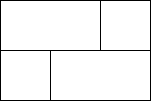
\includegraphics[scale=.3]{../solutions/2}
\par\vspace{1em}
$n = 3$\\
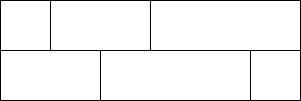
\includegraphics[scale=.3]{../solutions/3}
\par\vspace{1em}
$n = 4$\\
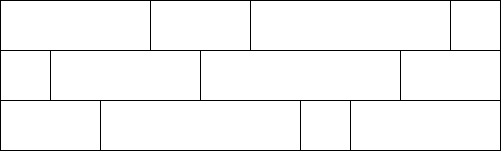
\includegraphics[scale=.3]{../solutions/4}
\par\vspace{1em}
$n = 5$\\
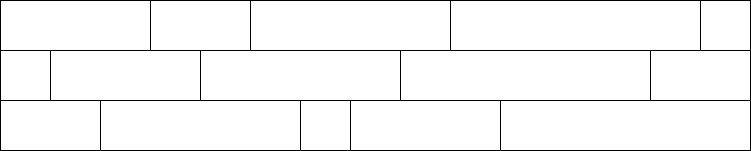
\includegraphics[scale=.3]{../solutions/5}
\par\vspace{1em}
$n = 6$\\
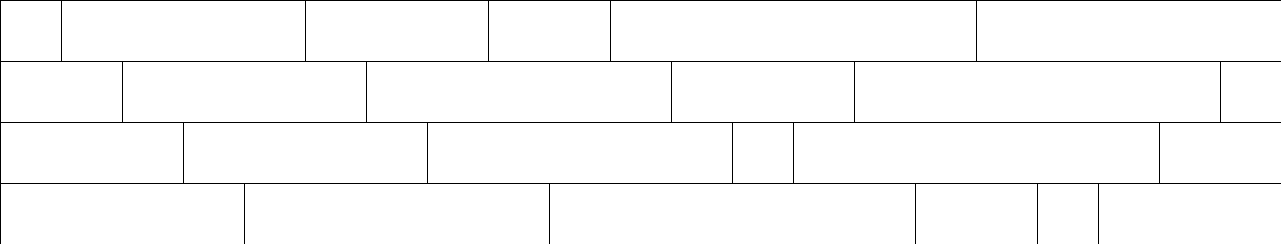
\includegraphics[scale=.3]{../solutions/6}
\par\vspace{1em}
$n = 7$\\
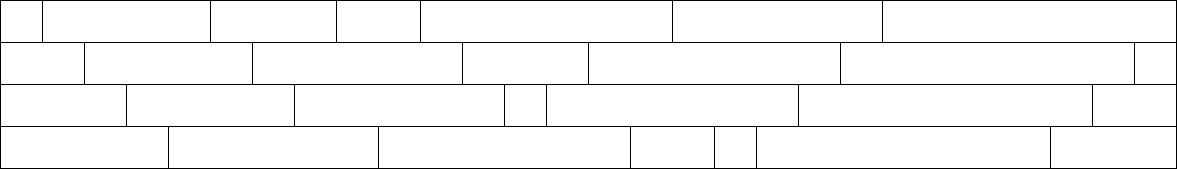
\includegraphics[width=\textwidth]{../solutions/7}
\par\vspace{1em}
$n = 8$\\
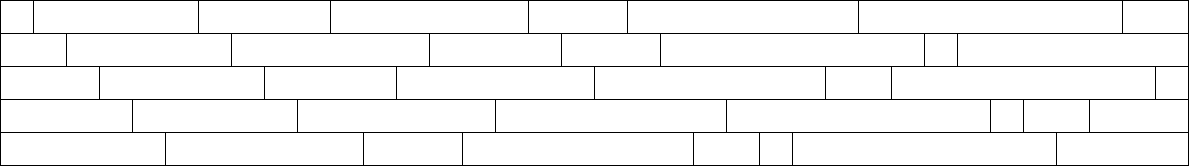
\includegraphics[width=\textwidth]{../solutions/8}
\par\vspace{1em}
$n = 9$\\
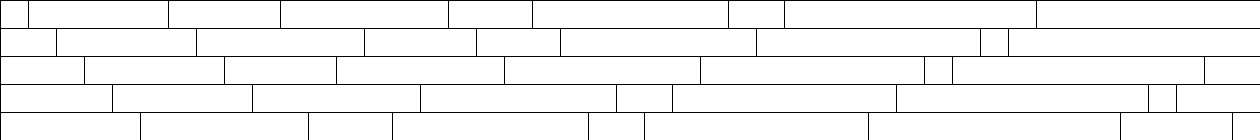
\includegraphics[width=\textwidth]{../solutions/9}
\par\vspace{1em}
$n = 10$\\
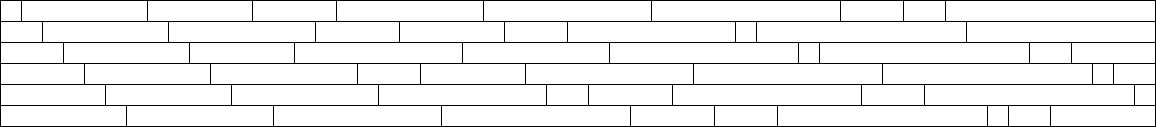
\includegraphics[width=\textwidth]{../solutions/10}
\par\vspace{1em}
$n = 11$\\
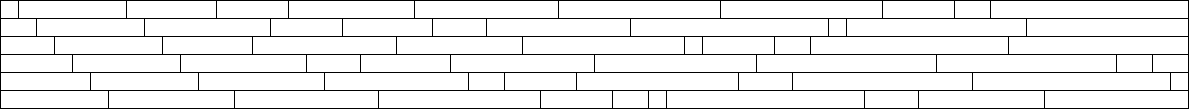
\includegraphics[width=\textwidth]{../solutions/11}
\par\vspace{1em}
$n = 12$\\
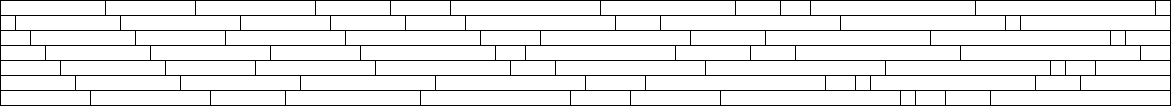
\includegraphics[width=\textwidth]{../solutions/12}
\par\vspace{1em}
$n = 13$\\
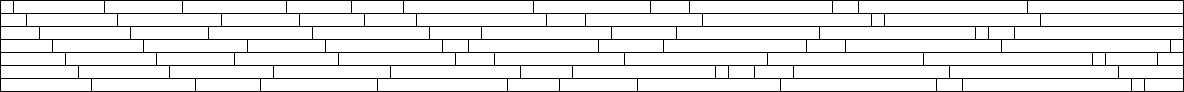
\includegraphics[width=\textwidth]{../solutions/13}
\par\vspace{1em}
$n = 14$\\
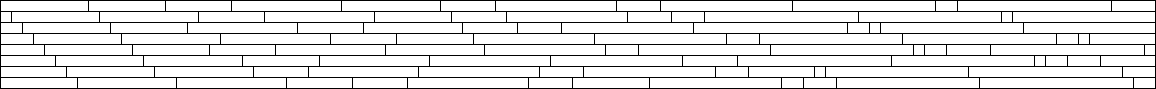
\includegraphics[width=\textwidth]{../solutions/14}
\par\vspace{1em}
$n = 15$\\
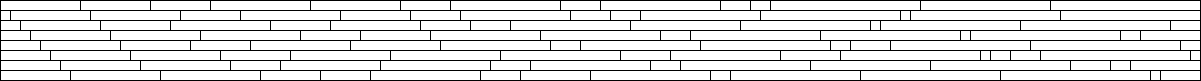
\includegraphics[width=\textwidth]{../solutions/15}
\par\vspace{1em}
$n = 16$\\
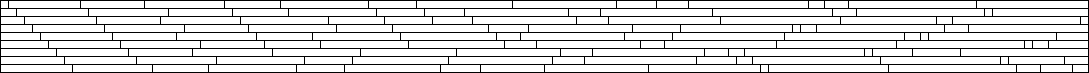
\includegraphics[width=\textwidth]{../solutions/16}
\par\vspace{1em}
\newpage
\subsubsection*{Text}
\vspace*{-1em}
\hspace{-10pt}
\texttt{
n = 2\\
1 2 \\
2 1\\
\\
n = 3\\
1 2 3 \\
2 3 1\\
\\
n = 4\\
1 3 2 4 \\
2 3 4 1\\
3 4 1 2\\
\\
n = 5\\
1 3 2 4 5 \\
2 3 4 5 1\\
3 4 1 5 2\\
\\
n = 6\\
1 4 3 2 6 5 \\
2 4 5 3 6 1\\
3 4 5 1 6 2\\
4 5 6 2 1 3\\
\\
n = 7\\
1 4 3 2 6 5 7 \\
2 4 5 3 6 7 1\\
3 4 5 1 6 7 2\\
4 5 6 2 1 7 3\\
\\
n = 8\\
1 5 4 6 3 7 8 2\\
2 5 6 4 3 8 1 7 \\
3 5 4 6 7 2 8 1\\
4 5 6 7 8 1 2 3\\
5 6 3 7 2 1 8 4\\
\\
n = 9\\
1 5 4 6 3 7 2 9 8\\
2 5 6 4 3 7 8 1 9 \\
3 5 4 6 7 8 1 9 2\\
4 5 6 7 2 8 9 1 3\\
5 6 3 7 2 8 9 4 1\\
\\
n = 10\\
1 6 5 4 7 8 9 3 2 10 \\
2 6 7 4 5 3 8 1 10 9\\
3 6 5 8 7 9 1 10 2 4\\
4 6 7 3 5 8 9 10 1 2\\
5 6 7 8 2 4 9 3 10 1\\
6 7 8 9 4 3 10 1 2 5\\
\\
n = 11\\
1 6 5 4 7 8 9 10 3 2 11 \\
2 6 7 4 5 3 8 11 1 10 9\\
3 6 5 8 7 9 1 4 2 11 10\\
4 6 7 3 5 8 9 10 11 1 2\\
5 6 7 8 2 4 9 3 10 11 1\\
6 7 8 9 4 2 1 11 3 10 5\\
\\
n = 12\\
1 7 6 8 5 4 10 9 3 2 11 12 \\
2 7 8 6 5 4 10 3 12 11 1 9\\
3 7 6 8 9 4 10 5 11 12 1 2\\
4 7 8 6 9 2 10 5 3 11 12 1\\
5 7 6 8 9 3 10 12 11 1 2 4\\
6 7 8 9 10 4 12 2 1 11 3 5\\
7 8 5 9 10 4 6 12 1 2 3 11\\
\\
n = 13\\
1 7 6 8 5 4 10 9 3 11 2 13 12\\
2 7 8 6 5 4 10 3 9 13 1 12 11\\
3 7 6 8 9 4 10 5 11 12 1 2 13 \\
4 7 8 6 9 2 10 5 11 3 12 13 1\\
5 7 6 8 9 3 10 11 12 13 1 4 2\\
6 7 8 9 10 4 11 1 2 3 12 13 5\\
7 8 5 9 10 4 6 11 12 2 13 1 3\\
\\
n = 14\\
1 8 7 6 10 9 5 11 4 12 13 2 14 3\\
2 8 9 6 10 7 5 11 4 3 14 13 1 12\\
3 8 7 10 6 9 5 4 12 14 2 1 13 11\\
4 8 9 10 6 7 11 12 3 13 14 2 1 5\\
5 8 7 6 10 9 11 3 12 13 1 2 4 14 \\
6 8 9 7 10 11 12 5 14 13 1 2 3 4\\
7 8 9 5 10 11 4 12 3 6 1 13 14 2\\
8 9 10 6 5 11 4 7 12 2 3 13 14 1\\
\\
n = 15\\
1 8 7 6 10 9 5 11 4 12 3 2 15 13 14\\
2 8 9 6 10 7 5 11 4 3 12 14 1 15 13\\
3 8 7 10 6 9 5 4 12 11 13 1 14 15 2\\
4 8 9 10 6 7 11 12 3 13 14 1 15 2 5\\
5 8 7 6 10 9 11 3 12 13 2 4 14 15 1\\
6 8 9 7 10 11 12 5 13 4 14 1 2 3 15 \\
7 8 9 5 10 11 4 12 3 13 14 15 1 2 6\\
8 9 10 6 5 11 4 7 12 2 13 14 15 1 3\\
\\
n = 16\\
1 9 8 10 7 11 6 12 13 5 4 15 2 3 16 14\\
2 9 10 8 7 11 6 5 13 4 14 15 3 16 1 12\\
3 9 8 10 11 7 6 5 13 4 14 15 12 2 16 1\\
4 9 10 8 11 7 12 5 13 6 14 1 2 16 3 15\\
5 9 8 10 7 11 12 3 13 6 14 15 2 1 16 4\\
6 9 10 8 7 11 12 4 13 3 14 15 16 1 2 5\\
7 9 8 10 11 12 13 4 14 3 2 15 1 5 6 16 \\
8 9 10 11 6 12 13 4 14 5 2 16 15 1 7 3\\
9 10 7 11 6 12 5 8 13 14 1 15 16 3 4 2\\
}

\newpage
\subsection*{Quellcode}
\lstinputlisting{../wall.cpp}
\end{document}